\documentclass{jsarticle}
\usepackage[dvipdfmx]{graphicx}
\usepackage{bm}
\usepackage{amsmath}
\usepackage{amssymb}
\usepackage{amsfonts}
\usepackage{comment}
\usepackage{listings}
\usepackage{cases}
\usepackage{siunitx}
\usepackage[hyphens]{url}
\lstset{
    basicstyle={\ttfamily},
    identifierstyle={\small},
    commentstyle={\smallitshape},
    keywordstyle={\small\bfseries},
    ndkeywordstyle={\small},
    stringstyle={\small\ttfamily},
    frame={tb},
    breaklines=true,
    columns=[l]{fullflexible},
    numbers=left,
    xrightmargin=0zw,
    xleftmargin=3zw,
    numberstyle={\scriptsize},
    stepnumber=1,
    numbersep=1zw,
    lineskip=-0.5ex,
    keepspaces=true,
    language=c
}
\renewcommand{\lstlistingname}{リスト}
\makeatletter
\newcommand{\figcaption}[1]{\def\@captype{figure}\caption{#1}}
\newcommand{\tblcaption}[1]{\def\@captype{table}\caption{#1}}
\makeatother

\title{MAC3Dによる運動の3D化}
\date{}

\begin{document}
    \maketitle
    \section{MAC3Dシステムの概要}
        MAC3Dは人体にマーカを貼り付け、
        専用のカメラを複数使い、運動の様子をすることでその動きを3D化する。

        \begin{figure}[h]
            \begin{minipage}{0.5\hsize}
                \centering
                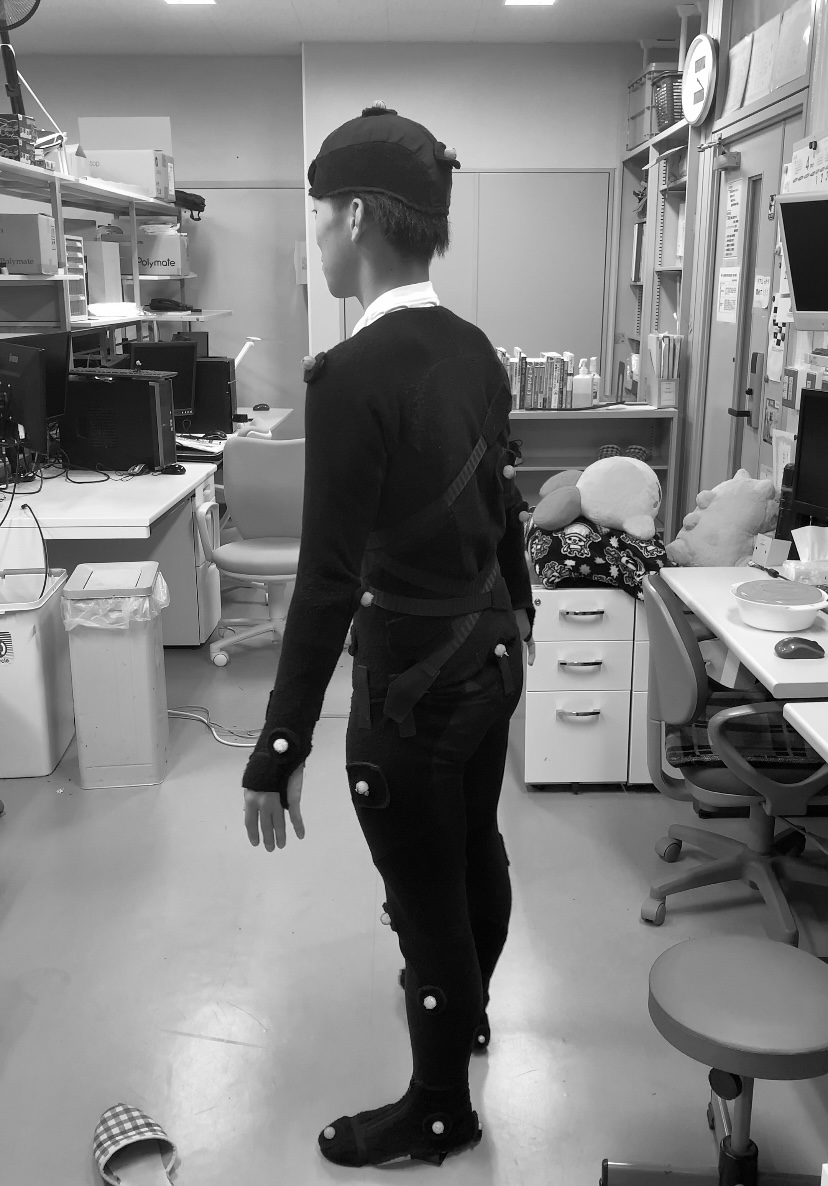
\includegraphics[width=0.9\hsize]{img/marker.jpg}
                \caption{被計測者の様子}
            \end{minipage}
            \begin{minipage}{0.5\hsize}
                \centering
                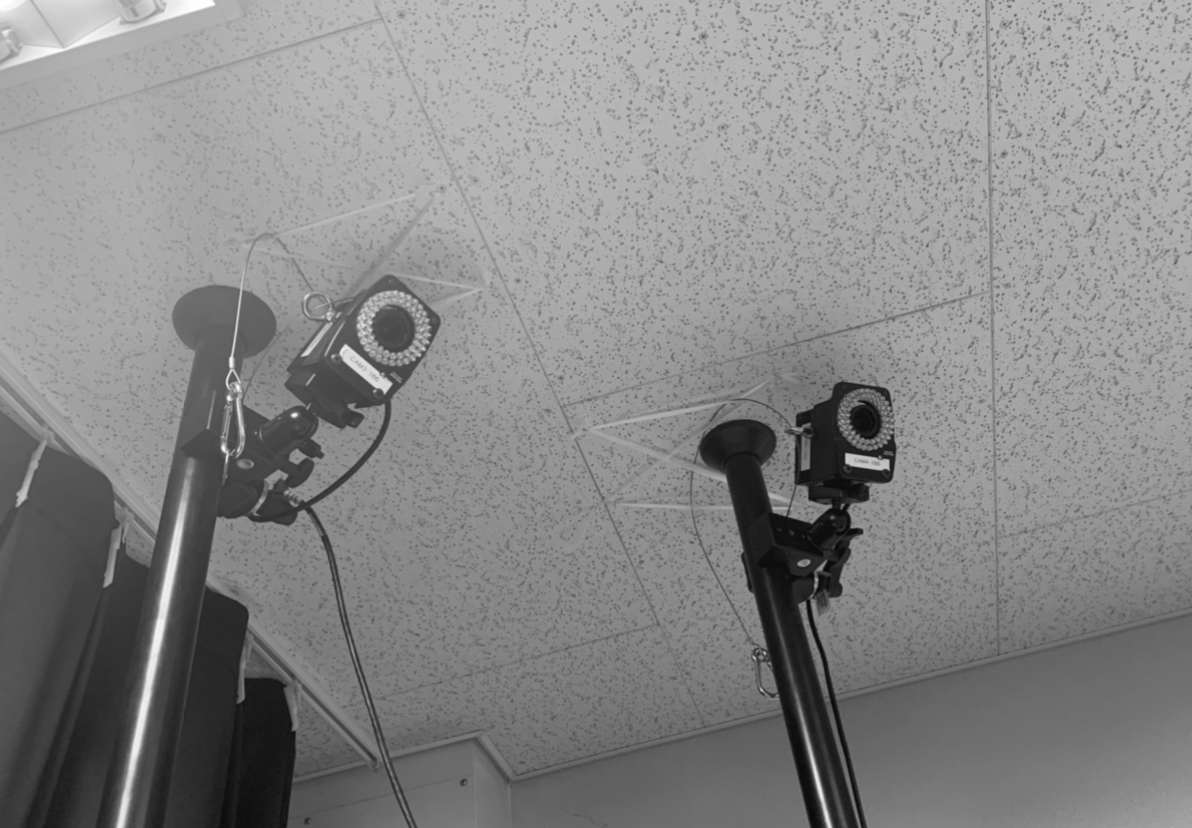
\includegraphics[width=0.9\hsize]{img/camera.jpg}
                \caption{計測に使用するカメラ}
            \end{minipage}
        \end{figure}

        図\ref{fig:data}にあるように、
        実際に被測定者がつけているマーカーがどのように動いていたかを計測できる。

        \begin{figure}[h]
            \centering
            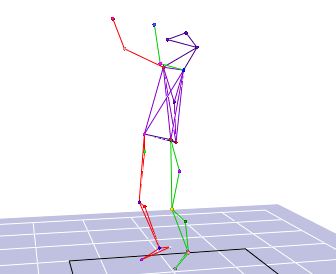
\includegraphics[width=0.6\hsize]{img/form.png}
            \caption{計測されたデータ}
            \label{fig:data}
        \end{figure}

    \section{動作の力学的解析}
        計測したデータから、より細かい解析を行うことができる。
        解析した結果を図\ref{fig:fujita}、\ref{fig:shuhei}に示す。

        \begin{figure}[h]
            \begin{minipage}{0.5\hsize}
                \centering
                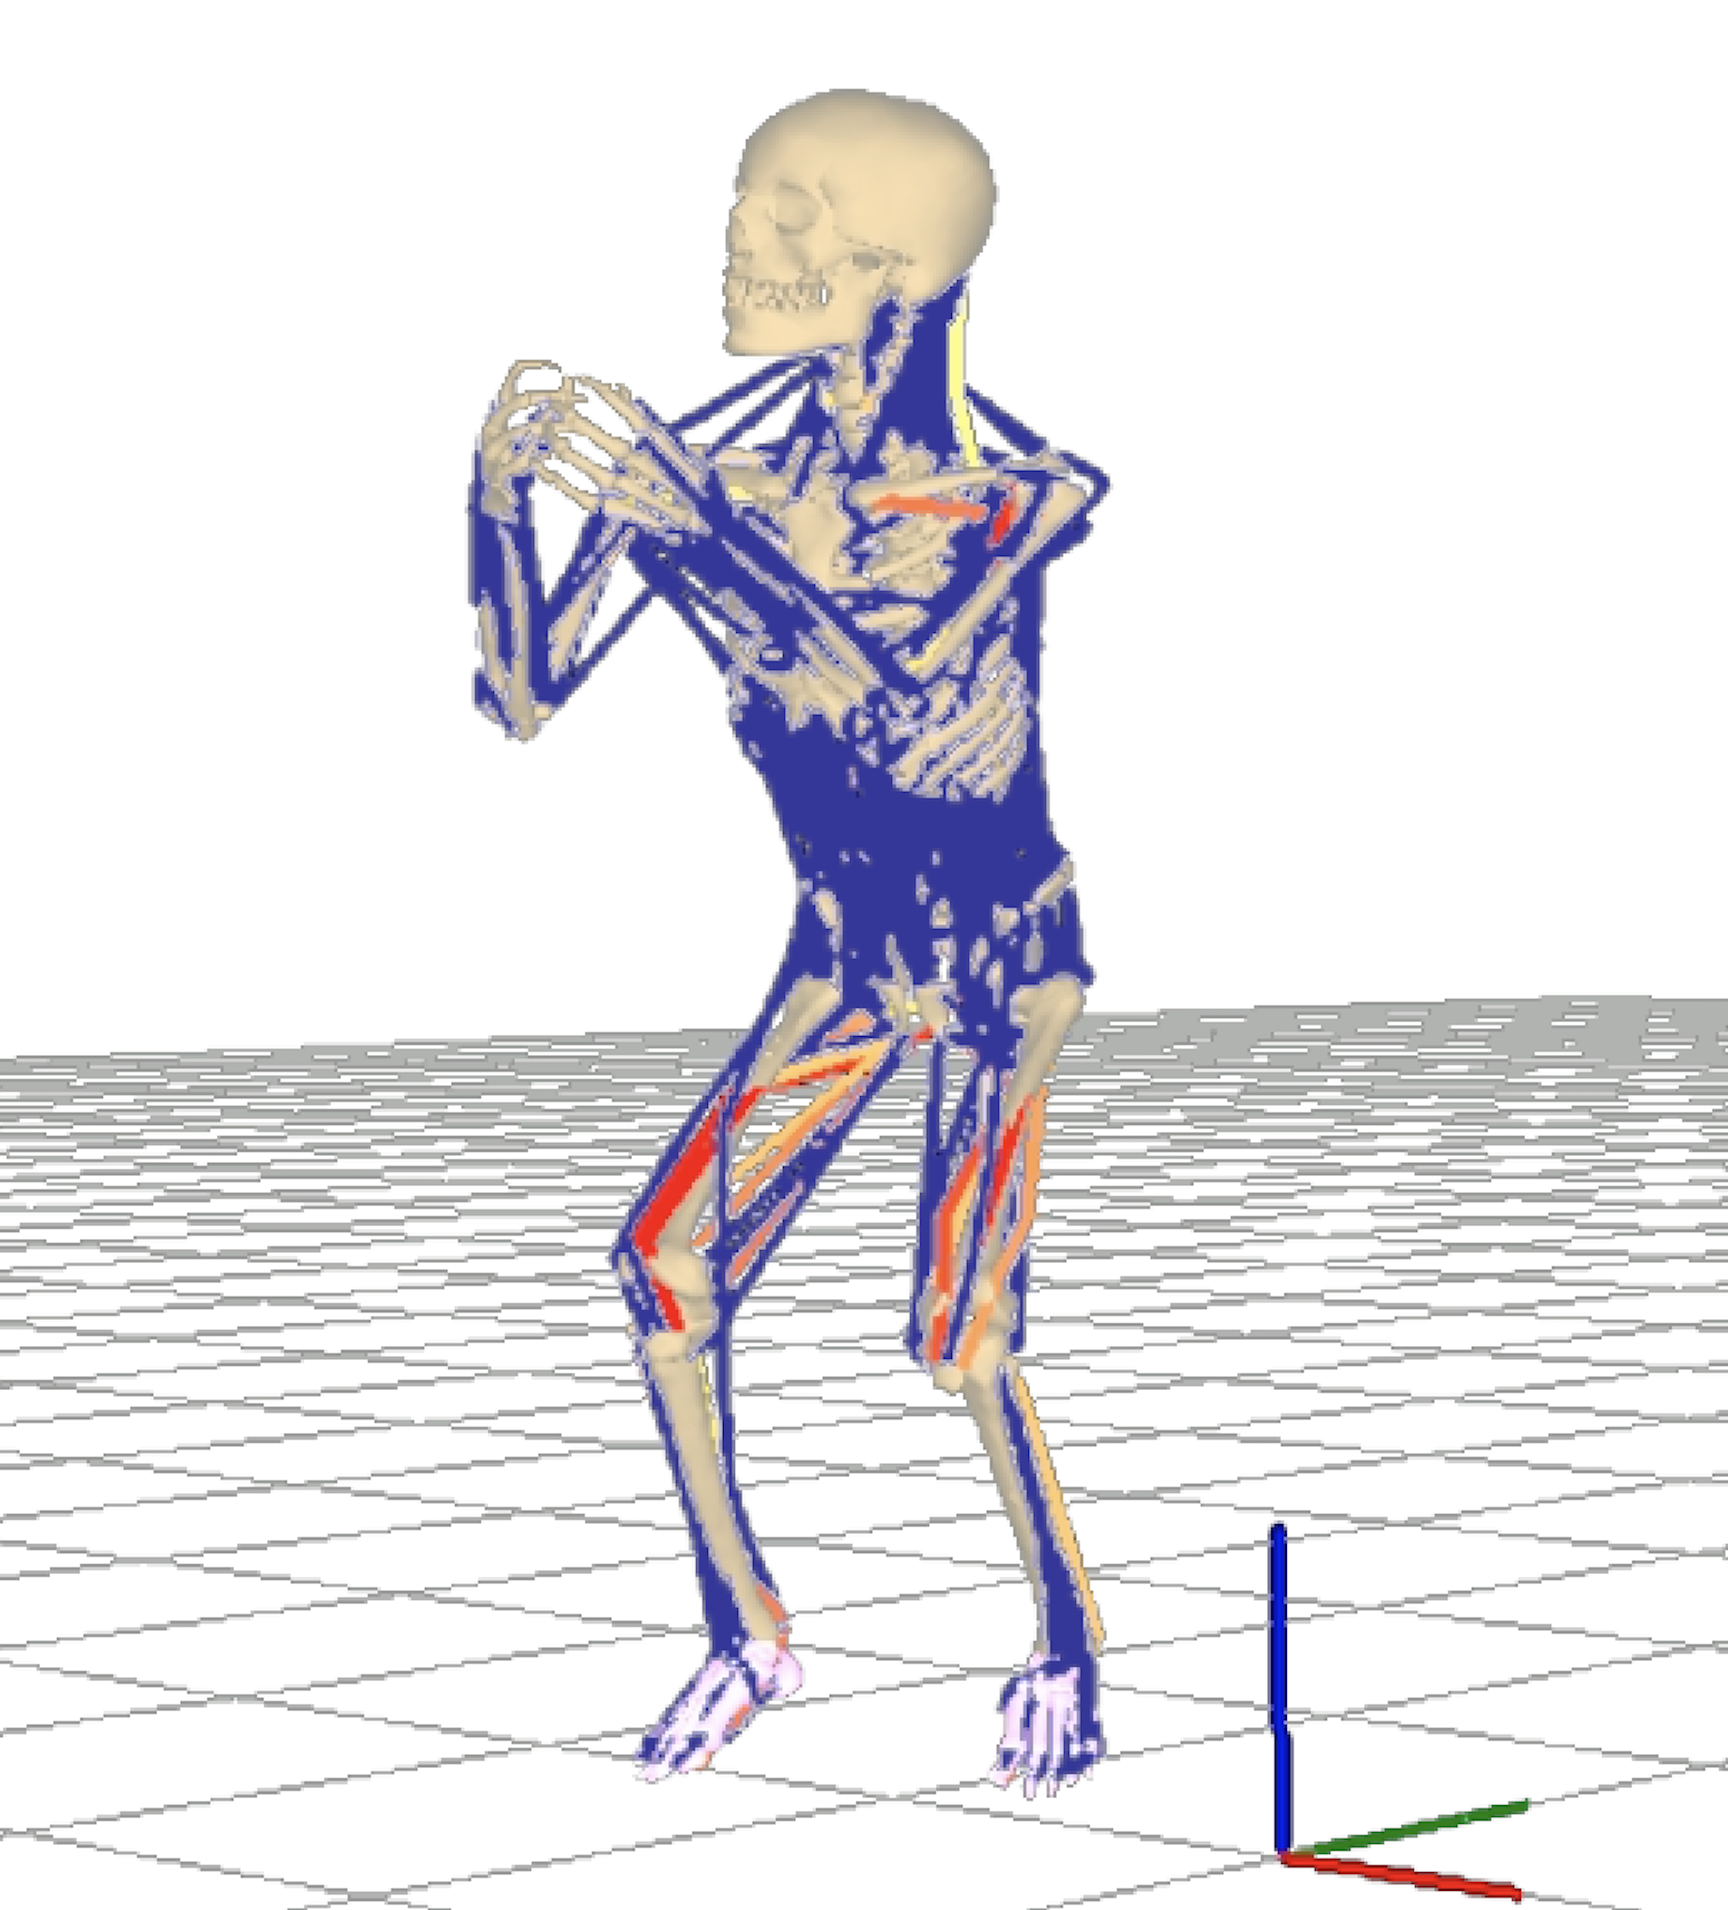
\includegraphics[width=0.9\hsize]{img/fujita.png}
                \caption{バスケ未経験者のフォーム}
                \label{fig:fujita}
            \end{minipage}
            \begin{minipage}{0.5\hsize}
                \centering
                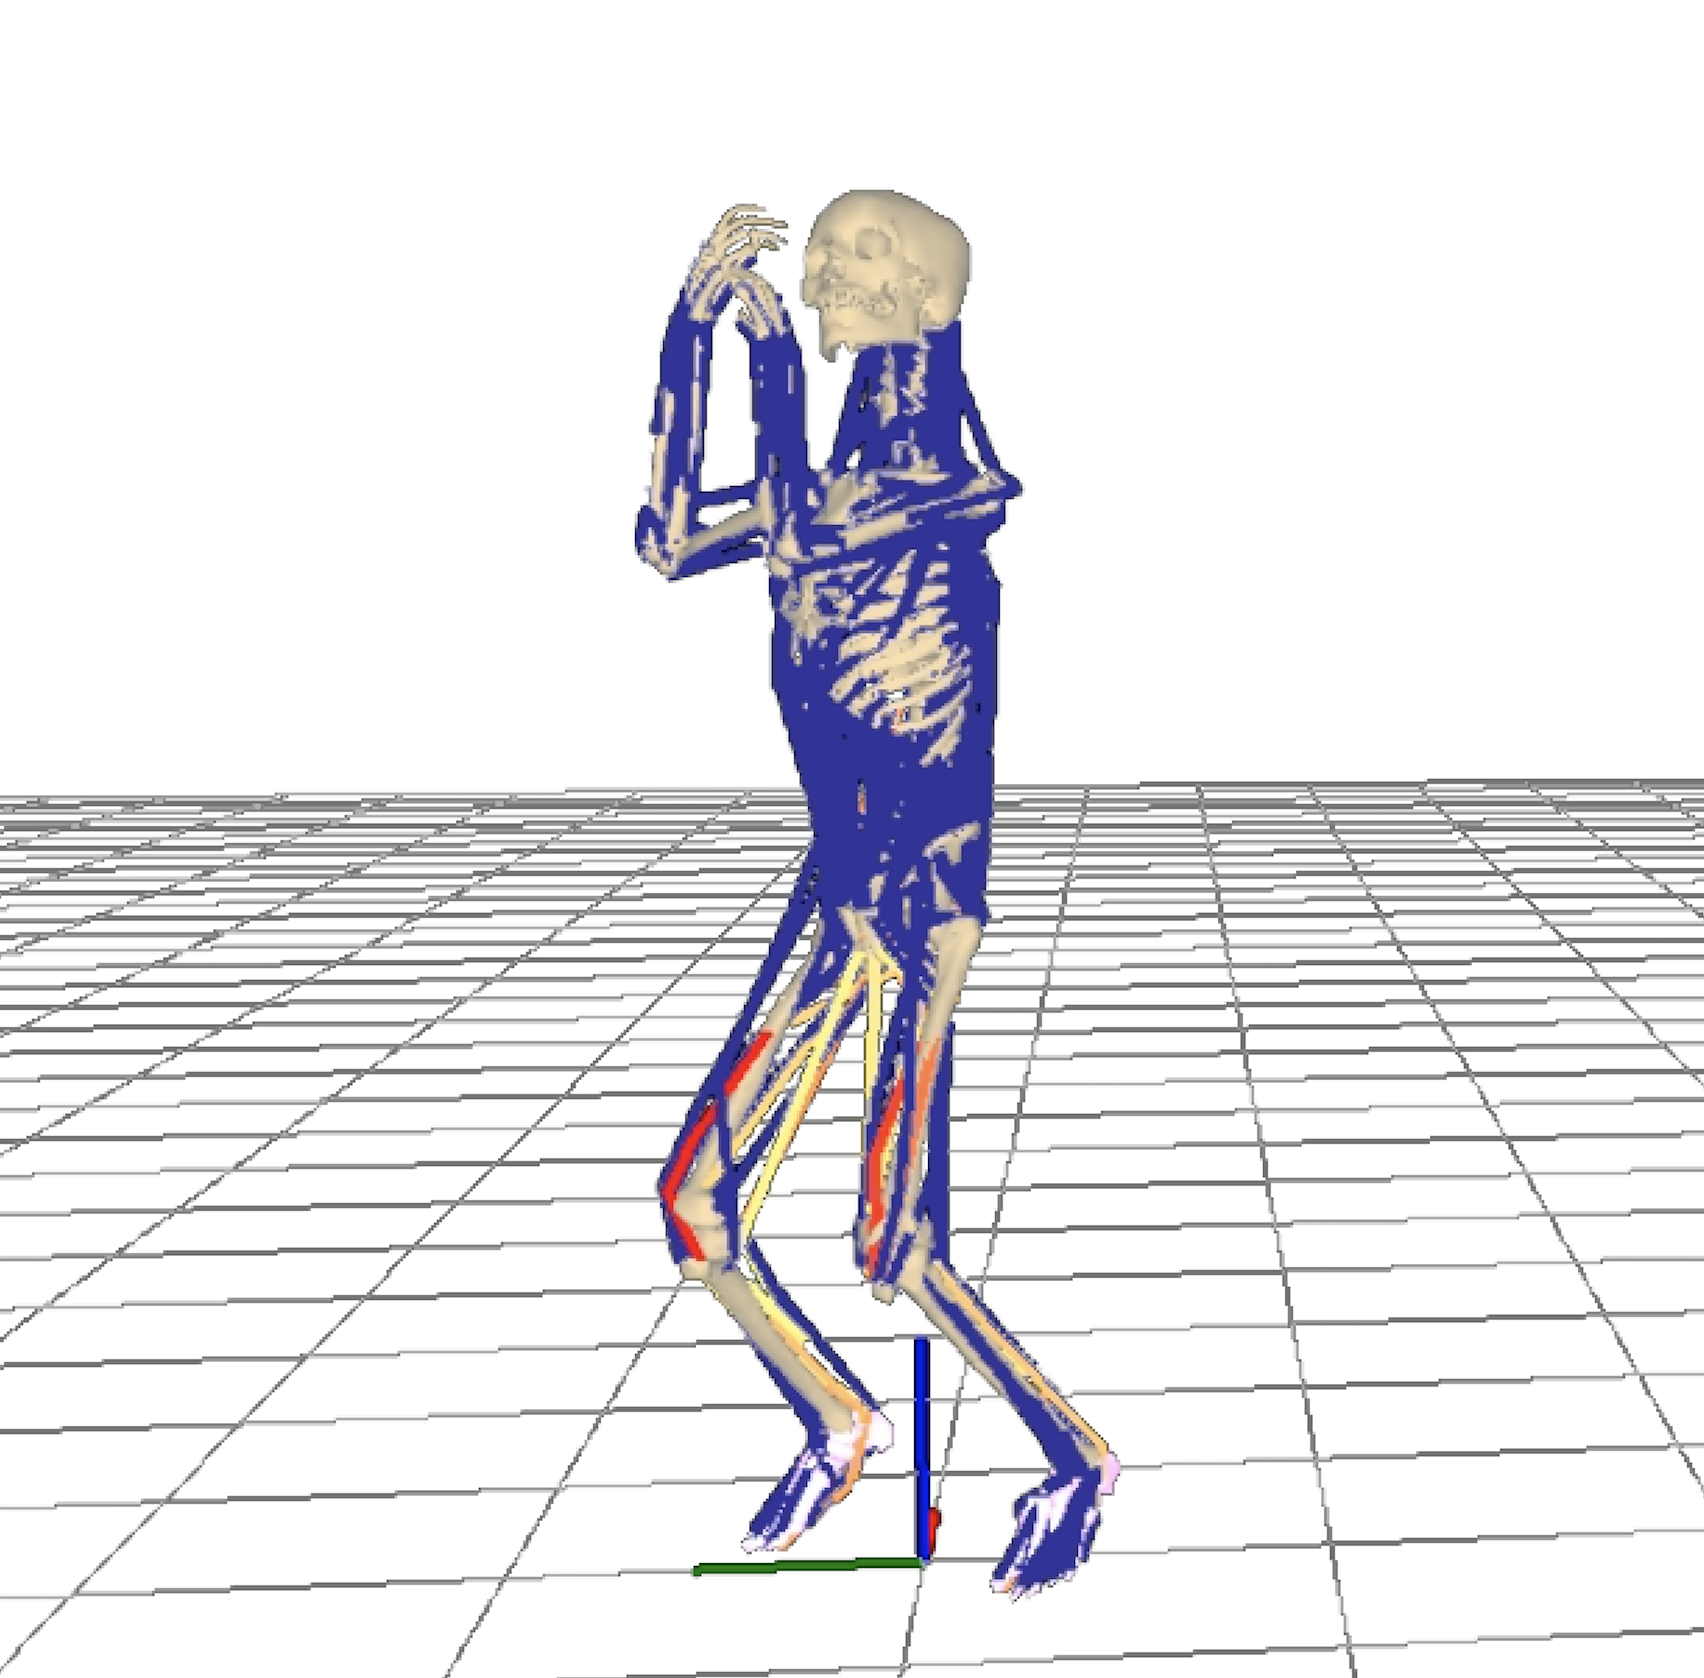
\includegraphics[width=0.9\hsize]{img/shuhei.png}
                \caption{バスケ経験者のフォーム}
                \label{fig:shuhei}
            \end{minipage}
        \end{figure}

        二つの図は、バスケ経験者と、未経験者それぞれのシュートの様子を解析したものである。

        紫の線が筋肉を示しており、力が入るほど黄色$\rightarrow$オレンジ$\rightarrow$赤
        と色が変わっている。
        二つの画像を比べることで、膝の曲がりや、力のかかっている場所などの差が見て取れる。

        また、実際の体の動きだけではなく、空中にいた時間や体の重心の移動なども検証することが可能である。

    \section{長・短所}
        最後に、MAC3Dシステムの長所と短所をそれぞれまとめる。

        \paragraph{長所}
            \begin{description}
                \item[精度] 筋肉、骨の動きなど詳細な解析ができる。
            \end{description}

        \paragraph{短所}
            \begin{description}
                \item[時間] 計測、解析ともに時間がかかる。リアルタイムでの実用は厳しい。
                \item[価格] 専用のカメラなど、機材が高価。
            \end{description}
\end{document}